In this chapter, product architecture is described using 4 + 1 architectural view model.
It is based on the multiple concurrent views and therefore better explanation of architecture can be provided.

\section{4 + 1 view model}
\subsection{Logical view}
The description of the functional requirements of the architecture. The client and the server are decomposed into a set of key abstractions, taken(mostly) from the problem domain, in the form of objects or object classes.

\subsection{Development view}
\subsection{Process view}

\begin{figure}[H]
	\centering
		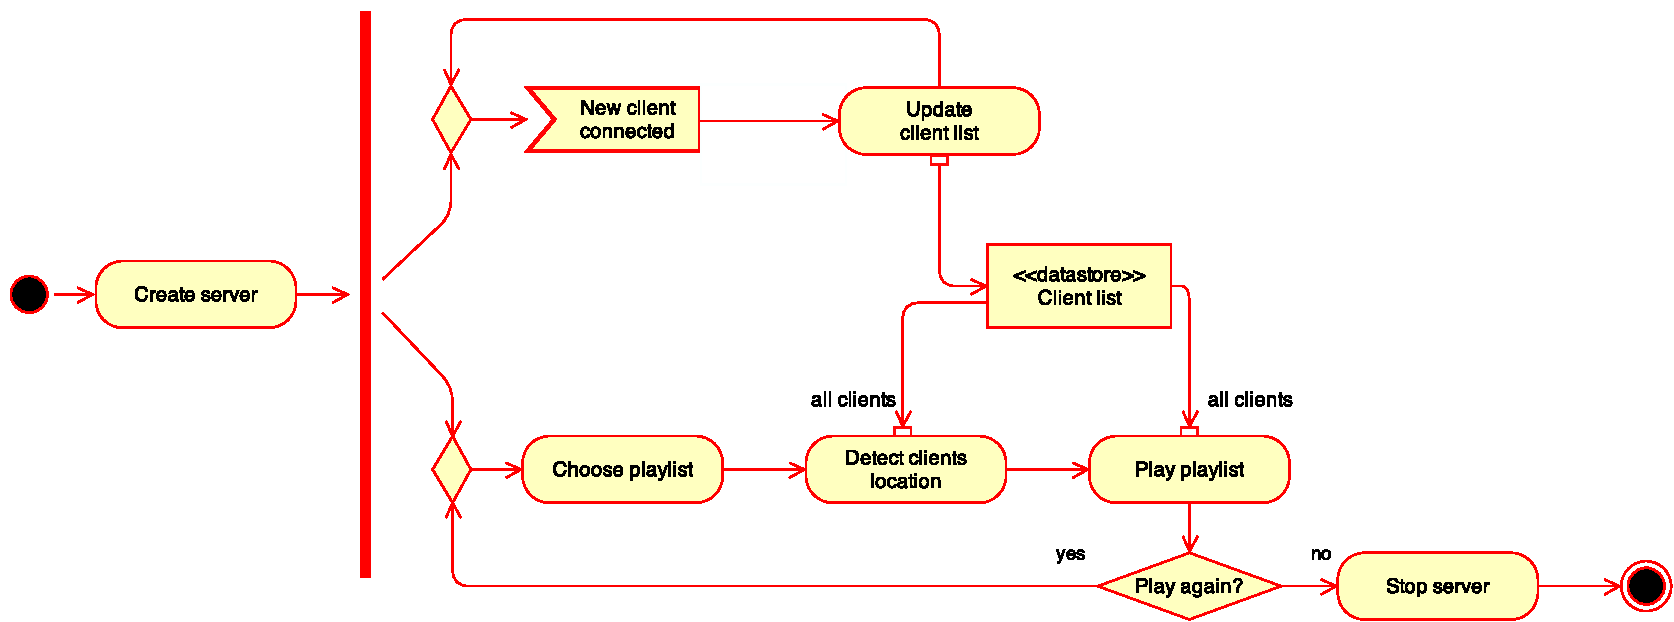
\includegraphics[width=16.2cm]{softwareArchitecture/activity_server.pdf}
	\caption{Activity diagram of server application}
	\label{fig:activity_diagram_server}
\end{figure}

\begin{figure}[H]
	\centering
		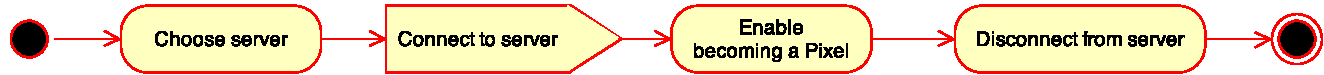
\includegraphics[width=16.2cm]{softwareArchitecture/activity_client.pdf}
	\caption{Activity diagram of client application}
	\label{fig:activity_diagram_client}
\end{figure}


\subsection{Physical view}
Physical view \cite{Kruchten:1995:VMA:624610.625529} describes a mapping of software onto hardware. 
It takes into account non-functional requirements of the system.

Physical view is described by deployment diagram \ref{fig:architecture_deployment_diagram}.
According to requirement \refreq{N1}, there are two executable files deployed; one deployed to client device and second to server device.
There is also need for NTP\footnote{http://ntp.org/} server, which will maintain all connected devices synchronized.
To generalize the architecture design, the \emph{camera} device is treated as a separate device, which will only send its output to server device.

\begin{figure}[H]
	\centering
		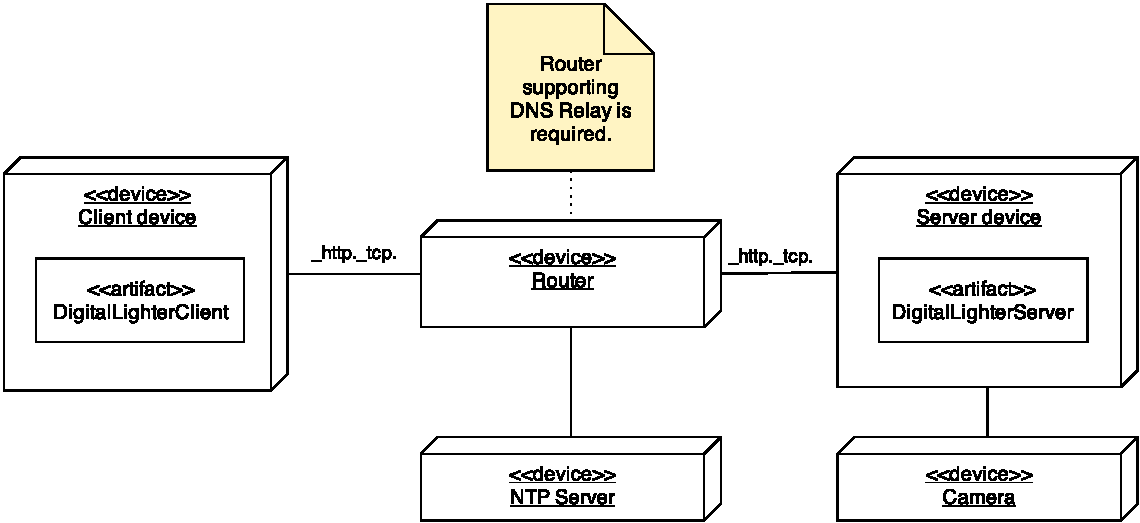
\includegraphics[width=15cm]{softwareArchitecture/deployment-diagram.pdf}
	\caption{Deployment diagram}
	\label{fig:architecture_deployment_diagram}
\end{figure}

\subsection{Scenarios}
Use case diagrams can be considered as scenarios, therefore introduced diagram \ref{img:usecase} in Requirements chapter can be considered as a scenario.

\section{Used design patterns}
\subsection{Strategy}
\subsection{Model-View-Controller}
\subsection{Observer}